% !TEX root =../dissertation.tex
\documentclass[./dissertation.tex]{subfiles}
\begin{document}
\chapter{Toward a Foundation Model for Biomedical Image Segmentation}
\label{ch:foundation}
\section{Introduction}

% 1. Supervised methods require large annotated data to perform well. Their generalizability suffers. \\
% 2. Unsupervised methods are good in that they don't need a lot of annotated data, but their accuracy is not as good and they can be very domain-specific. \\

Biomedical image segmentation is pivotal across a diverse array of medical and biological applications, from diagnostic imaging to cellular analysis. While supervised segmentation methods, especially convolutional neural networks (CNNs), have achieved remarkable accuracy, their reliance on large, annotated datasets severely limits their generalizability and transferability, particularly in biomedical contexts where labeled data is scarce and costly to obtain. Conversely, unsupervised methods, despite being simpler and more generalizable, often fall short in segmentation precision and robustness, thus failing to meet the accuracy requirements of clinical and research settings.


% 3. foundation models are trained on very large datasets. SAMs are good at zero-shot segmentation for they learn the repesentation of textures, objects, etc. they can take in prompts in the form of bounding boxes and points. these SAMs can potentially be a good easy to use choice for producing good-enough masks. \\
% 4. How SAMs work. the internal mechanism that allows it to take points and generage masks. or just generate masks for all objects in the image. \\
% 5. SAM struggles with biomedical images since it is originally trained on general images (e.g. horse, cat, cat, etc.). that's why it needs to be fine-tuned to be able to perform reliably for biomedical images. \\

Recently, the emergence of Foundation Models (FMs) and the Segment Anything Model (SAM) offers a compelling new direction for addressing these limitations. SAM, introduced by Kirillov et al. \cite{kirillov2023segment}, marked a significant advancement by achieving impressive zero-shot segmentation capabilities across varied image domains, relying only on minimal user prompts such as points or bounding boxes. Its successor, SAM 2, further extends these capabilities into video segmentation, leveraging advanced architectures to improve accuracy and interaction efficiency \cite{ravi2024sam}. These models are trained on large and diverse datasets, enabling them to generalize effectively across multiple segmentation tasks without extensive domain-specific training. Despite their potential, the application of general-purpose SAM models to biomedical imaging presents unique challenges. The complex and nuanced nature of biomedical images characterized by varying imaging modalities, structures, textures, and noise levels means that models trained primarily on general-domain images may struggle to achieve desirable segmentation accuracy \cite{mazurowski2023segment,na2024segment}. Recognizing this, adaptations of SAM tailored specifically to biomedical contexts have emerged. Models such as MedSAM \cite{ma2024segment} and MediViSTA-SAM \cite{kim2025medivista} demonstrate the feasibility of adapting SAM to medical imaging and video analysis, showing promising results that often surpass specialized, modality-specific models in robustness and accuracy.



% 6. There are many biomedical adaptations for SAM, including this and that and the other one which do this and that and something else, each of which focusing on improving some aspect of SAM. They all show that their work has promising improvements. \\

% 7. There's another set of research done on incorporating text prompts into SAM. it involves training text-image pairs first and the model uses contrastive learning to clusterize or localize the similar text-image embeddings. CLIP is a famous model. in inferrence, this CLIP model takes the prompt and image and tries to highlight the locations on the image which it finds relevant to the prompt. then some random points or bounding boxes are created using this heatmap and then passed to SAM for downstream segmentation. there are of course some biomedical adaptations of CLIP like BiomedCLIP. they perform great vs. the vanilla CLIP. \\


% 8. But there is so much stochasticity and randomness within this process. from the way the CLIP model is trained or fine-tuned to how this inference is done and how the point and box prompts are selected. they all affect the final outcome of the SAM's mask decoder. \\

Alongside spatial segmentation capabilities, the integration of vision-language models like BiomedCLIP \cite{zhang2023biomedclip} into SAM workflows has gained considerable attention. BiomedCLIP, trained on extensive biomedical image-text pairs, provides robust multimodal embeddings that bridge textual and visual domains, enabling powerful text-driven segmentation. Frameworks such as MedCLIP-SAMv2 exemplify this integration, demonstrating how textual prompts can effectively guide precise segmentation tasks, from identifying tumors in medical scans to delineating specific cellular structures in microscopy images. However, the integration of vision-language models with SAM introduces additional layers of complexity and stochasticity. Variability in outputs stemming from factors such as the fine-tuning process of models like BiomedCLIP, differences in textual prompts, or randomness in inference strategies can undermine reproducibility, a critical factor in biomedical research and clinical applications. Thus, understanding and mitigating this stochasticity is paramount for the practical adoption and reliability of these models.

% 9. that's why we're focusing on this part, aiming to find ways to control this randomness and increase the reproducibility of the CLIP, hence helping SAM in honing in on the ROI that best matches the prompt.

This chapter aims to comprehensively explore and address these challenges. We focus specifically on evaluating and enhancing the reproducibility of integrated vision-language segmentation models, investigating how different factors—including fine-tuning strategies, prompt engineering, and inference methodologies—influence variability in segmentation outcomes. Our goal is to develop methodologies that standardize and optimize these variables, ensuring SAM-based models are not only accurate and versatile but also reliably reproducible in biomedical contexts.

\section{Background}

% 1. SAM's original paper, and the subsequent SAM2. \\

SAM \cite{kirillov2023segment} introduced a groundbreaking promptable segmentation approach, trained on a vast dataset (SA-1B), featuring over one billion masks. Its architecture comprises three components: a powerful Vision Transformer (ViT) image encoder, a flexible prompt encoder handling points, boxes, and text, and a lightweight mask decoder to produce segmentation masks. SAM's notable innovation lies in its zero-shot capabilities achieved through prompt engineering, enabling it to generalize well across various segmentation tasks, even without task-specific fine-tuning. SAM-2 \cite{ravi2024sam} extends SAM's capabilities to video data, incorporating a memory attention mechanism that retains information from previous frames, thereby significantly enhancing segmentation accuracy and interaction efficiency. SAM-2 utilizes a hierarchical transformer architecture (Hiera) \cite{ryali2023hiera,bolya2023window} pre-trained with masked autoencoders (MAE) \cite{he2022masked}, making it highly effective for real-time segmentation tasks across images and videos. This memory-enhanced architecture allows SAM-2 to iteratively refine masks, leading to considerable improvements in temporal segmentation consistency. A comprehensive survey titled "Foundation Models for Biomedical Image Segmentation" \cite{lee2024foundation} underscores the transformative potential of SAM, summarizing over 100 studies that have successfully adapted SAM to a wide range of biomedical datasets. The survey highlights SAM's strong zero-shot capabilities and outlines various domain-specific tuning methods and data scarcity challenges that have driven innovation in biomedical segmentation.


% 2. Biomedical adaptations of SAM and what they focus on. \\

The success of the SAM in general-domain image segmentation has inspired adaptations and methodological enhancements aimed at tailoring its capabilities specifically for biomedical applications, addressing unique challenges associated with medical image segmentation. MedSAM \cite{ma2024segment} and other models, like BioSAM-2 \cite{yan2024biomedical}, have demonstrated the necessity of domain-specific fine-tuning for achieving clinical-grade accuracy. BioSAM-2, particularly designed for biomedical segmentation, has optimized SAM-2 with medical domain-specific data and additional memory mechanisms for improved performance across diverse biomedical imaging modalities. Medical SAM Adapter (Med-SA) \cite{wu2023medical} introduced adaptation modules such as Space-Depth Transpose (SD-Trans) and Hyper-Prompting Adapter (HyP-Adpt), which enhance SAM's performance on medical images through minimal yet strategic parameter adjustments. These modules have shown significant improvements over traditional segmentation methods by efficiently incorporating medical domain knowledge.

In the realm of prompt learning and auto-prompting the Segment Any Cell (SAC) \cite{na2024segment} framework leveraged auto-prompting and fine-tuning methods, using Low-Rank Adaptation (LoRA) \cite{hu2022lora}, to automatically generate effective prompts for nuclei segmentation. This method reduced manual intervention and improved segmentation accuracy in microscopic imaging scenarios. SSPrompt \cite{huang2024learning} optimized SAM's spatial and semantic prompts directly within its embedding space, enhancing its generalization capabilities across complex segmentation tasks. The Segment and Caption Anything \cite{huang2024segment} model enriched SAM's semantic understanding capabilities by integrating a query-based feature mixer, improving semantic precision and enabling the model to provide meaningful regional captions, thus enhancing segmentation results through better semantic contextualization.



% 3. Biomedical adaptations of CLIP. some researches matched the best description to the image. some other did other things. \\

% Incorporation and Integration of Text Prompts in Biomedical SAM
% a. Vision-Language Models and Multi-Modal Integration
The support for textual prompts in the original SAM is relatively limited and experimental compared to spatial (points, boxes, masks) prompts. Building upon the advancements in adapting SAM for biomedical tasks, recent research has increasingly focused on incorporating text prompts and integrating vision-language models to further enhance segmentation precision and semantic interpretability in medical imaging. Models like BiomedCLIP \cite{zhang2023biomedclip} and adaptations such as MedCLIP-SAMv2 \cite{koleilat2024medclipsamv2, koleilat2024medclip} underscore the importance of text-driven segmentation approaches, leveraging extensive biomedical image-text pairs to provide robust multimodal embeddings. This integration enables powerful and precise segmentation guided by textual descriptions, thus bridging visual and textual biomedical data effectively. The EVF-SAM \cite{zhang2024evf} model exemplifies the integration of early vision-language fusion. It incorporates an early fusion mechanism, significantly outperforming late fusion models by enhancing text-to-image attention, which is critical for accurate segmentation guided by referring expressions.

% b. Specific Applications and Advancements in Text-guided Biomedical Segmentation
Polyp-SAM++ \cite{biswas2023polyp} demonstrated the effectiveness of detailed textual prompts specifically for colorectal polyp segmentation, showing how text guidance could substantially improve the segmentation accuracy and robustness of SAM, particularly in clinically relevant contexts . Hi-SAM \cite{ye2024hi} extended SAM's capabilities to hierarchical text segmentation, including pixel-level text, word, text-line, and paragraph segmentation, thus enabling more structured and detailed biomedical image analyses, crucial for applications like pathology slide examination. PROMISE \cite{li2024promise} and similar models have adapted SAM to 3D biomedical segmentation, introducing lightweight adapters for depth-related spatial context and achieving superior performance in tumor segmentation tasks by effectively combining textual prompts with depth-awareness.

% 4. Universal Segmentation and Multi-Modal Integration for Enhanced Biomedical Analysis
The Segment Anything with Text prompts (SAT) \cite{zhao2023one} model, trained on an extensive dataset comprising over 22,000 medical scans and nearly 500 anatomical classes, exemplifies a universal segmentation framework that integrates extensive medical terminologies as textual prompts. This approach emphasizes the utility of incorporating domain-specific knowledge directly into the model training, significantly improving segmentation performance across diverse medical imaging tasks.

When using text-to-segmentation pipelines, segmentation results should ideally be deterministic given the same input. However, randomness can creep in through various stages, both at inference and during training. There is growing interest in modeling the stochasticity and uncertainty inherent in medical image segmentation. In practice, what constitutes the "correct" segmentation can be ambiguous – different experts may trace slightly different boundaries for the same lesion, especially in low-contrast or complex cases \cite{rakic2024tyche}. Models like SAM produce one deterministic mask per prompt, which doesn't capture this ambiguity, however, this ambiguity is maximised when incorporating text-to-segment pipelines, since the text-image input of the CLIP should be transformed into spacial points to be fed to SAM as input prompts. In MedCLIP-SAMv2 \cite{koleilat2024medclip} this step is done with the help of extracting attention maps of BiomedCLIP given a text-image pair. This saliency map highlights the locations of interest in the image which are then used to select points or bounding boxes for SAM.

% In this article we take MedCLIP-SAMv2 to be the ground of our research and attempt to understand the impacting factors and parameters to the reproducibility of the attention maps of the text-image encoder. We will investigate how effective each of these 

Our methodology builds upon the principles of MedCLIP-SAMv2, integrating the BiomedCLIP vision-language model with SAM to improve segmentation accuracy and reproducibility in biomedical applications. Initially, we evaluate the baseline capability of BiomedCLIP to differentiate various biological structures, emphasizing its performance on complex and previously unseen entities such as ciliary regions. Subsequently, we explore the impact of fine-tuning BiomedCLIP, examining how variations in fine-tuning parameters influence its effectiveness. Lastly, we assess multiple strategies for selecting optimal spatial prompts as inputs for SAM, aiming to identify methods that consistently yield accurate segmentation outcomes.
%  specifically in detecting ciliary regions from nasal epithelial biopsy videos. 

\section{Methodology}
% 1. my methodology involves fine-tuning BiomedCLIP on the dataset of cilia i have. the cilia dataset contains videos or nasal epithelial biopsy containing ciliary regions. these videos are annotated and the annotations show where the body of the cell is and where the ciliary region are. sometimes the ciliary region sticks out of the boundary of the cell which makes them easy to detect with eye and some other times they overlap the body of the cell or are out of focus which makes them very hard to detect even by human. anyway. I finetune the BiomedCLIP model using masked images of cell bodies and masked images of cilia along with their respective textual descriptions and then use the model to infer on unseen data. my aim is to find out which factors undermine the reproducibility of this process. those are: fine-tuning the model and for how long and how much, the text descriptions of the patches, whether using masked images or raw images, and - finally when the BiomedCLIP spits out a heatmap of its predictions - what's the best strategy in selecting positive/negative points or bounding boxes considering the output of the BiomedCLIP - that is going to be the input of SAM - to make sure we get accurate and reproducible results

This chapter outlines a systematic approach developed to enhance segmentation accuracy and reproducibility in biomedical imaging, specifically targeting the segmentation of ciliary regions in nasal epithelial biopsy videos. Leveraging the BiomedCLIP vision-language model integrated with the SAM, the methodology involves fine-tuning BiomedCLIP on a specialized dataset containing annotated videos of nasal epithelial biopsies. These annotations distinctly mark cell bodies and associated ciliary regions, which vary significantly in visibility—ranging from clearly delineated, easily identifiable structures to overlapping and out-of-focus regions challenging even to expert human annotators. The methodology rigorously explores how different fine-tuning parameters, textual prompts, and image pre-processing strategies (masked versus raw) influence BiomedCLIP's performance. Subsequently, the trained BiomedCLIP generates predictive heatmaps on previously unseen data, serving as a basis for strategically selecting spatial prompts for SAM segmentation. Finally, this research investigates various prompt selection strategies to determine optimal methods for ensuring consistent, accurate, and reproducible segmentation results.



\subsection{Datasets}

\subsubsection{Cilia Dataset}
Our principal dataset comprises 681 microscopy videos of nasal epithelial biopsies, among which 325 videos have detailed annotations. Each video depicts epithelial cells exhibiting either normal motile cilia, dyskinetic (immotile) cilia. Annotated masks explicitly identify three types of regions: cell bodies, clearly visible cilia structures, and overlapping, hard-to-detect cilia. Visible cilia typically extend beyond cell boundaries, appearing clearly against a blank background, thus facilitating their straightforward identification in static frames. Conversely, overlapping cilia structures, often oriented vertically toward the microscope lens or appearing sparse and out of focus, pose significant detection challenges, even to human annotators. Such challenging structures usually require observing subtle rhythmic patterns across video frames for confident identification.

For simplicity and consistency within our methodology, both visible and overlapping ciliary regions were grouped into a single class termed "ciliary structure." To evaluate the effectiveness of fine-tuning BiomedCLIP and subsequent segmentation using SAM, the annotated cilia dataset was split into training and testing subsets following a 70/30 ratio.
% The cilia dataset comprises annotated videos highlighting cell bodies and ciliary regions, which vary significantly in visibility and overlap, presenting unique detection challenges.

\subsubsection{The Cell Tracking Challenge Dataset \cite{mavska2023cell}:}
We employed selected datasets from the Cell Tracking Challenge (CTC), which offers a comprehensive collection of 2D and 3D time-lapse microscopy images, each representing diverse biological organisms and imaging modalities. These datasets cover a broad range of specimens, including human, mouse, rat, Caenorhabditis elegans, Drosophila melanogaster, and others, captured using modalities such as Brightfield, Differential Interference Contrast (DIC), and Fluorescence microscopy (detailed in Table 2.1). Given the relative uniformity of image slices within individual datasets, a small representative sample from each was sufficient for benchmarking BiomedCLIP's inherent segmentation capabilities prior to fine-tuning.

\subsubsection{BiomedCLIP Model}
% BiomedCLIP has been combined with SAM in models like MedCLIP-SAMv2, where BiomedCLIP generates saliency maps or text-based feature maps that guide SAM's segmentation process. This integration allows text-driven segmentation (e.g., segmenting "tumor region" based on a natural language prompt), opening doors to more interactive and automated medical image analysis. BiomedCLIP is a multimodal foundation model designed for biomedical image and text understanding. It is a contrastive vision-language model trained on 15 million biomedical image-text pairs extracted from PubMed Central. The model learns joint representations of biomedical images and their textual descriptions, enabling it to perform various medical vision-language tasks.
% BiomedCLIP is based on OpenAI's CLIP (Contrastive Language–Image Pretraining) but adapted for biomedical data. Its training follows the standard CLIP contrastive learning pipeline:

% Image encoder: A vision transformer (ViT-B/16 or ViT-L/14) processes images.
% Text encoder: A transformer-based language model (PubMedBERT) encodes corresponding biomedical text descriptions.
% Contrastive learning: The model learns to map similar images and text closer in embedding space while pushing unrelated pairs apart.
% Unlike vanilla CLIP, which was trained on general images (e.g., cats, landscapes, objects), BiomedCLIP is trained specifically on biomedical data, allowing it to capture domain-specific features crucial for tasks like radiology, histopathology, and medical illustrations.

BiomedCLIP, a contrastive vision-language model tailored specifically for biomedical domains, integrates effectively with segmentation frameworks like SAM, exemplified by models such as MedCLIP-SAMv2. Trained on 15 million biomedical image-text pairs from PubMed Central, BiomedCLIP leverages a vision transformer (ViT) for image encoding and PubMedBERT \cite{gu2021domain} for text encoding. Through contrastive learning, it aligns related images and textual descriptions into a joint embedding space. Unlike general-purpose models like CLIP \cite{radford2021learning}, BiomedCLIP captures nuanced, domain-specific features, making it uniquely suited for precise biomedical image analysis tasks, including saliency-driven segmentation.

\begin{figure}[h]
    \centering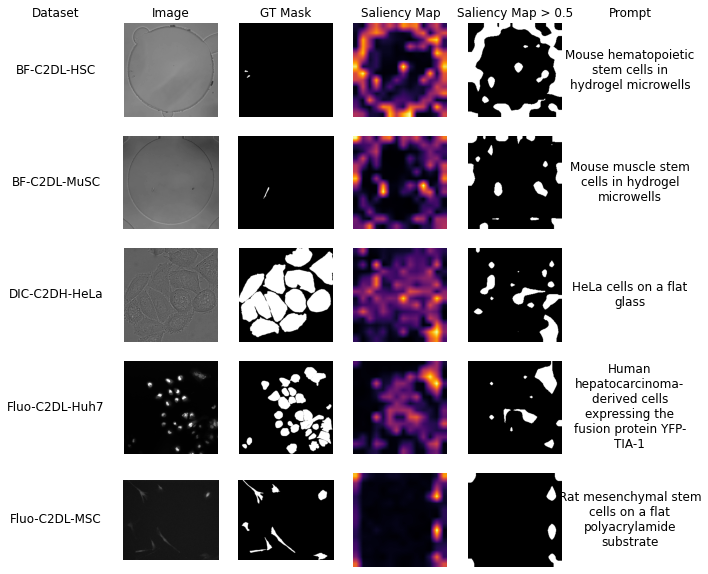
\includegraphics[width=.48\textwidth]{figures/sam/untuned1.png}
    \centering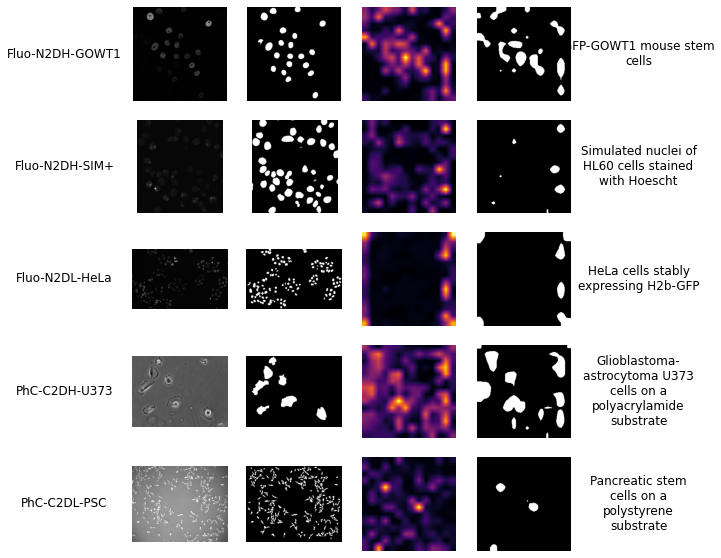
\includegraphics[width=.48\textwidth]{figures/sam/untuned2.png}
    \caption{BiomedCLIP's out-of-the-box performance over CTC's 2D datasets}
    \label{fig:untuned}
\end{figure}

Figure \ref{fig:untuned} shows the off the shelf performance of BiomedCLIP over 2D datasets in CTC.


\subsubsection{Fine-Tuning Strategies}
% Fine-tuning is done on BiomedCLIP's pretrained \(BiomedCLIP-PubMedBERT_256-vit_base_patch16_224\) model in batches of size 32, and \(1e-3\) as the learning reate, weight decay set to 0.1, for 32 epochs, using DHN-NCE loss introduced in MedCLIP-SAMv2. Model checkpoints are saved after each epoch.

% we changed these parameters in fine-tuning for the cilia dataset: 1. tuning for less/more epochs. 2. tuning with raw images vs. training with masks of cells and cilia. 3. tuning with long descriptions vs. short descriptions. 4. tuning by varying loss funciton parameters.


To investigate the impact of different fine-tuning parameters on BiomedCLIP's performance for cilia segmentation, we systematically varied several key factors. These included adjusting the number of training epochs, comparing fine-tuning on raw images versus masked images (isolating cell bodies and ciliary structures), utilizing varying lengths of textual descriptions as noted in Table \ref{tab:caption_generation_logic} (short versus detailed versus randomized detailed annotations), and experimenting with different configurations of loss function parameters. The parameter variations are summarized in Table~\ref{tab:fine-tune-params}.

\begin{table}[ht]
    \caption{Fine-Tuning Parameter Variations}
    \centering
    \label{tab:fine-tune-params}
    \begin{tabular}{|l|l|}
        % \toprule
        \hline
        \textbf{Parameter}       & \textbf{Variation Descriptions}                           \\  \hline
        Number of Epochs         & 2 epochs vs. 32 epochs                                    \\ \hline
        Input Images             & Raw images vs. Masked images                              \\ \hline
        Textual Descriptions     & Concise vs. Detailed Vs. Randomized detailed descriptions \\ \hline
        Loss Function Parameters & Default settings vs. Adjusted weighting schemes           \\ \hline
        % \bottomrule
    \end{tabular}
\end{table}
% (\texttt{BiomedCLIP-PubMedBERT\_256-vit\_base\_patch16\_224})
The fixed parameters for fine-tuning included the pretrained BiomedCLIP model, a batch size of 32, learning rate of \(1\times10^{-3}\), weight decay of 0.1, training duration of 32 epochs, and the DHN-NCE loss introduced in MedCLIP-SAMv2. Model checkpoints were saved after each epoch.



\subsubsection{DHN-NCE Loss Function}
% The Decoupled Hard Negative Noise Contrastive Estimation (DHN-NCE) loss is an enhancement of the standard InfoNCE loss used in contrastive learning. It is designed to mitigate issues such as the negative-positive-coupling (NPC) effect, which reduces learning efficiency, especially for small batch sizes. DHN-NCE achieves this by:
% \begin{itemize}

%     \item Decoupling positive samples from the denominator of the contrastive loss, improving optimization.
%     \item Incorporating hard negative sampling, which gives more importance to difficult negative samples, improving model learning.

% \end{itemize}
% The loss is computed separately for image-to-text \((Lv \rightarrow t)\) and text-to-image \((Lt \rightarrow v)\) contrastive learning and then summed:


The Decoupled Hard Negative Noise Contrastive Estimation (DHN-NCE) loss is designed to improve contrastive learning by decoupling positive samples from the denominator and introducing hard negative sampling. The loss function consists of two terms: one for image-to-text learning and another for text-to-image learning. Table \ref{tbl:param_change_effect} describes the effects of increasing or decreasing each of the loss-function parameters.


\paragraph{Loss Definition\\}

The overall DHN-NCE loss is defined as:
\begin{equation}
    L_{\text{DHN-NCE}} = L_{v \to t} + L_{t \to v}
\end{equation}

Each term is computed as follows:

\begin{equation}
    L_{v \to t} = -\sum_{i=1}^{B} \frac{I_{p,i} T_{p,i}^\top}{\tau} + \sum_{i=1}^{B} \log \left( \sum_{j \neq i} e^{I_{p,i} T_{p,j}^\top / \tau} W_{v \to t} \right)
\end{equation}

\begin{equation}
    L_{t \to v} = -\sum_{i=1}^{B} \frac{T_{p,i} I_{p,i}^\top}{\tau} + \sum_{i=1}^{B} \log \left( \sum_{j \neq i} e^{T_{p,i} I_{p,j}^\top / \tau} W_{t \to v} \right)
\end{equation}

where:
\begin{itemize}
    \item \( I_{p,i} \) and \( T_{p,i} \) are the normalized image and text features.
    \item \( B \) is the batch size.
    \item \( \tau \) is the temperature parameter controlling the sharpness of the distribution.
    \item \( W_{v \to t} \) and \( W_{t \to v} \) are hardness weights for negative samples.
\end{itemize}

\paragraph{Hardness Weighting Factors\\}

The hardness weighting factors are defined as:

\begin{equation}
    W_{v \to t} = (B-1) \times \frac{e^{\beta_1 I_{p,i} T_{p,j}^\top / \tau}}{\sum_{k \neq i} e^{\beta_1 I_{p,i} T_{p,k}^\top / \tau}}
\end{equation}

\begin{equation}
    W_{t \to v} = (B-1) \times \frac{e^{\beta_2 T_{p,i} I_{p,j}^\top / \tau}}{\sum_{k \neq i} e^{\beta_2 T_{p,i} I_{p,k}^\top / \tau}}
\end{equation}


\begin{table}
    \caption{Effects of parameter changes on DHN-NCE loss.}
    \centering
    % \renewcommand{\arraystretch}{1.2}
    \label{tbl:param_change_effect}
    \begin{tabular}{|c|c|c|}
        \hline
        \textbf{Parameter}                & \textbf{Effect of Increasing}           & \textbf{Effect of Decreasing}          \\
        \hline
        Temperature (\( \tau \))          & Smoother similarity distribution        & Sharper contrast, possible instability \\
        \hline
        Hardness (\( \beta_1, \beta_2 \)) & Emphasizes difficult negatives          & Less focus on hard negatives           \\
        \hline
        Positive Weight (\( \alpha \))    & More weight on positives, less contrast & Stronger negative differentiation      \\
        \hline
    \end{tabular}
\end{table}


\subsubsection{Evaluation of BiomedCLIP Predictions}

To quantitatively assess the accuracy of the generated heatmaps, a thresholding method was required prior to computing evaluation metrics such as Dice coefficient and Intersection over Union (IoU) against ground-truth masks. Our experiments indicated that the threshold selection critically influences the evaluation outcomes, and the optimal threshold value differs markedly across various fine-tuning configurations. Specifically, models with minimal or no fine-tuning necessitated relatively lower thresholds, whereas models subjected to extensive fine-tuning required comparatively higher thresholds to achieve optimal segmentation performance.


\section{Results and Discussion}

% Figure \ref{fig:untuned_garbage_results} depicts the performance of off-the-shelf BiomedCLIP over a sample of our cilia dataset. The same prompts were used during inference for all sample images. \textit{short}, \textit{med}, and \textit{detailed} prompts correspond to \textit{"respiratory cilia"}, \textit{"cilia on nasal epithelial cells"}, and \textit{"normal or abnormal cilia in nasal epithelial biopsy. some cilia are sticking out of the border of the cell making them visible, some other are overlapping the cell making them harder to detect"}. un-tuned BiomedCLIP struggled to detect ciliary regions.




% our experiments showed that fine-tuning the model on full images severely damages the accuracy of the model making it incapable of localizing the region of interest in any of the test. we performed fine-tuning for 2 and 32 epochs and the results were the same, although the heatmaps generated after 32 epochs were lighting up more specific regions.

% training on full size vs small size didn't make any difference.
% more epochs = throwing weight off
% training with validation set causes overfitting and the model to perform terribly.
% short descriptions + short prompts were more consistent. long descriptions led to more false positives and false negatives.
% no significant impact for changing beta 1 or 2.
% increasing temperature or alpha = no significant difference except throwing the model off on some hard to detect cilia on some images.
% increasing both temp and alpha produced inconsistency and reduced reproducibility.

% --temperature-dhnnce 0.1  --alpha-dhnnce 0.9  --beta1-dhnnce 0.95  --beta2-dhnnce 0.05  more sensitive to text prompt differences. med prompts were terrible

% --temperature-dhnnce 0.1 \
% --alpha-dhnnce 0.9 \
% --beta1-dhnnce 0.95 \
% --beta2-dhnnce 0.05 and long captions while training + short prompts

% --temperature-dhnnce 0.1 \
% --alpha-dhnnce 0.9 \
% --beta1-dhnnce 0.65 \
% --beta2-dhnnce 0.65 and long captions = best performance. more ability to detect different points. less false negatives more false positives.

% --temperature-dhnnce 0.1 \
% --alpha-dhnnce 0.9 \
% --beta1-dhnnce 0.95 \
% --beta2-dhnnce 0.15 i think the best is training with long captions prompting with short texts

% \subsubsection{varying prompts}
% short to the point prompts =less errors i.e. less false positives, more aligned with RoI
% training on short captions requires short prompts. training on long captions work better with more detailed prompts.



% This study systematically evaluated the performance of BiomedCLIP for generating saliency maps used to generate spatial prompts for SAM over our dataset of nasal epithelial cells containing ciliary regions. The experiments were designed to explore critical factors affecting accuracy and reproducibility, including fine-tuning duration, image processing methods (raw vs. masked), and textual prompts.


To establish a baseline performance for localizing ciliary regions in nasal epithelial biopsy images, the off-the-shelf BiomedCLIP model was evaluated without domain-specific fine-tuning. Textual prompts of varying lengths were used during inference: \textit{Short} ("respiratory cilia"), \textit{Medium} ("cilia on nasal epithelial cells"), and \textit{Detailed} ("normal or abnormal cilia in nasal epithelial biopsy...harder to detect"). As qualitatively illustrated in Figure \ref{fig:untuned_garbage_results}, the un-tuned model struggled to consistently and accurately identify ciliary structures, often generating saliency maps poorly aligned with the ground truth masks. Quantitative metrics calculated from thresholded saliency maps corroborated these limitations. While average IoU and Dice scores across test samples are presented in Table \ref{tab:biomedclip_performance}, visual inspection and individual sample metrics revealed that IoU scores for specific predictions rarely exceeded 0.01, underscoring the challenges faced by the un-tuned model and motivating the need for fine-tuning. It is also important to note that threshold selection significantly impacts these metrics, adding complexity to direct comparisons based solely on average scores.

\begin{figure}
    \centering
    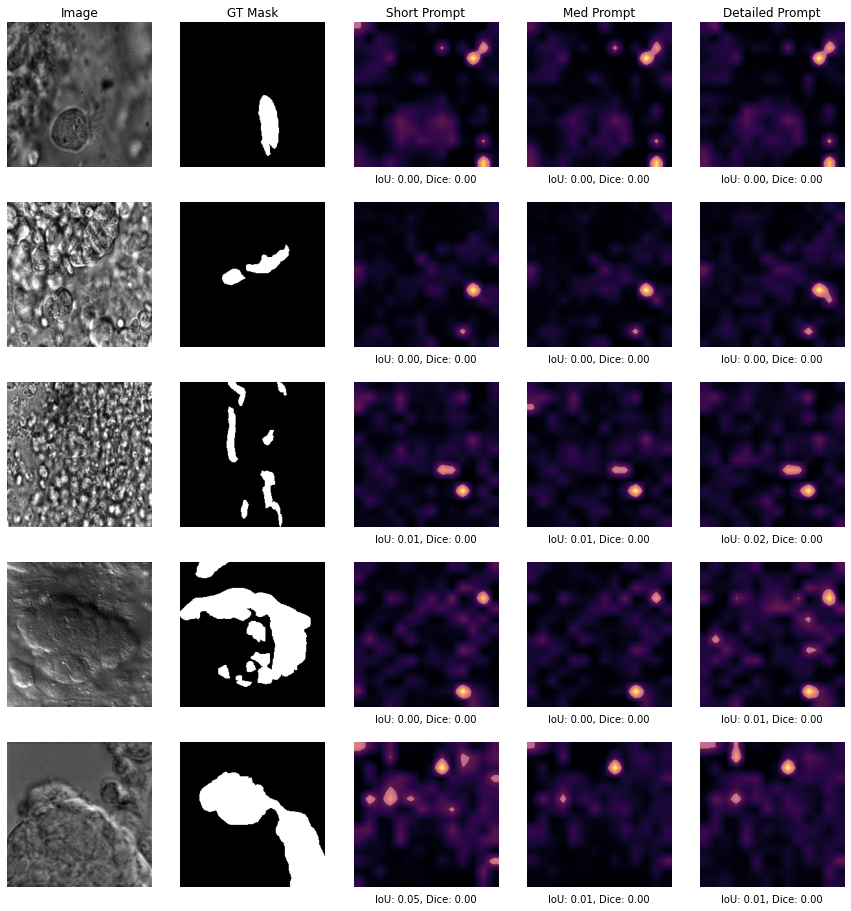
\includegraphics[width=0.4\textwidth]{figures/sam/untuned garbage results.png}
    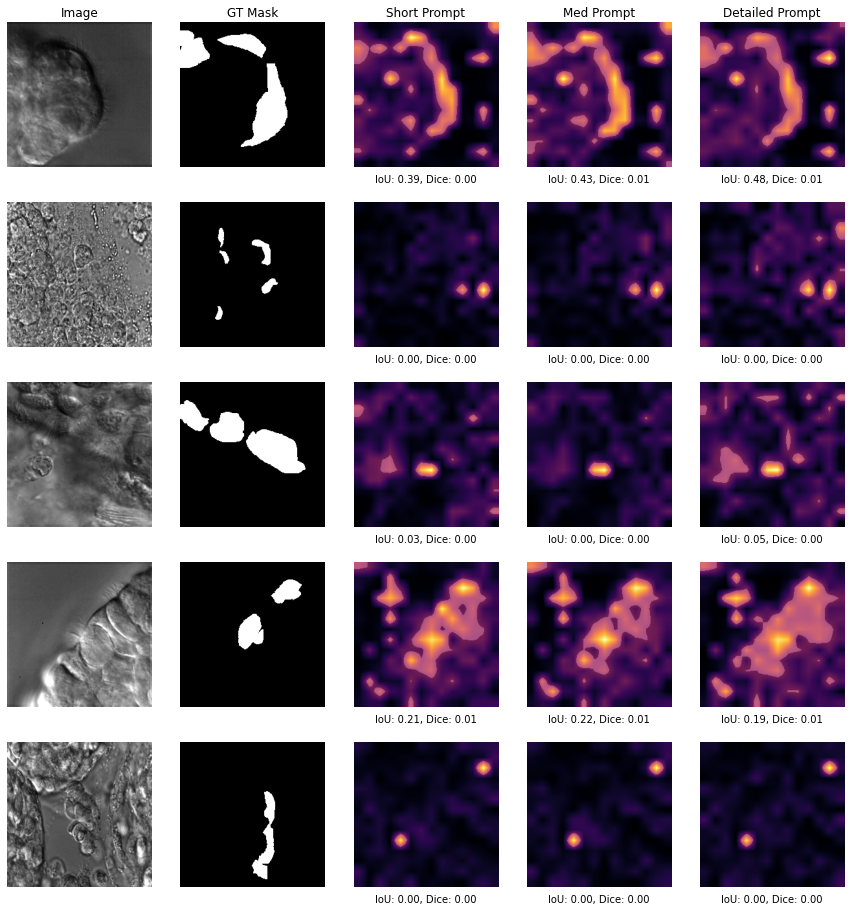
\includegraphics[width=0.4\textwidth]{figures/sam/untuned short med long.png} % Assuming this shows similar untuned results or is intended to be part of the comparison
    \caption{Performance of off-the-shelf BiomedCLIP with Short, Medium, and Detailed prompts, demonstrating poor localization without fine-tuning.}
    \label{fig:untuned_garbage_results}
\end{figure}

\begin{figure}
    \centering
    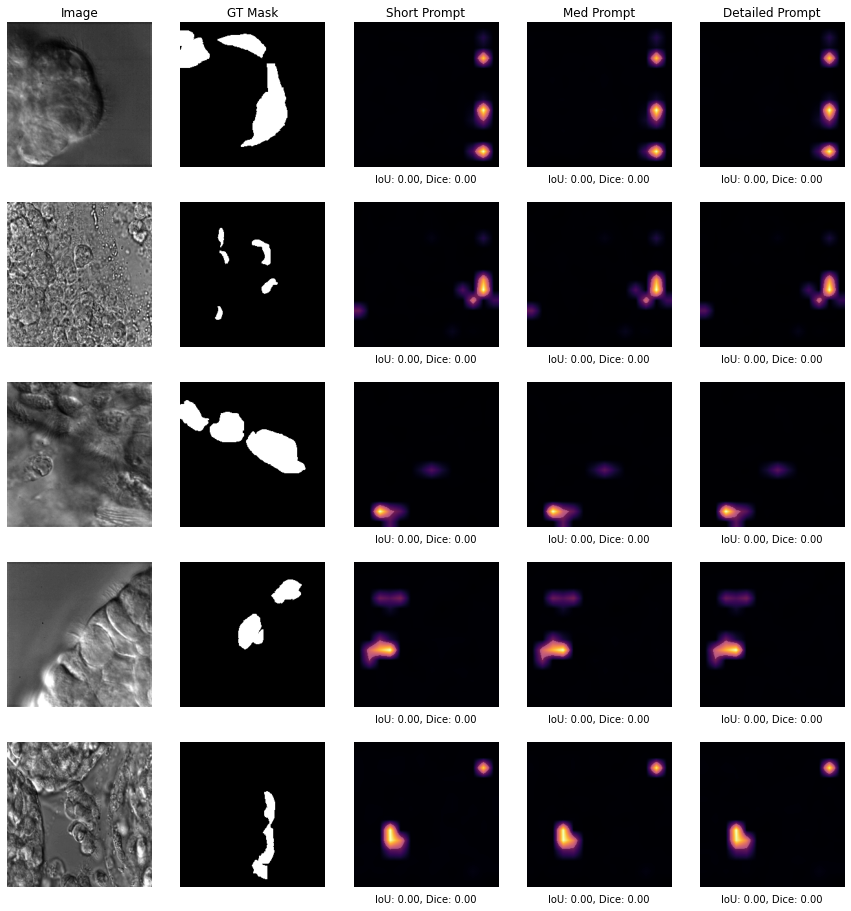
\includegraphics[width=\textwidth]{figures/sam/fine-tuned no mask ep 32.png}
    \caption{Localization results after fine-tuning BiomedCLIP for 32 epochs on full images without masks, showing incorrect and overly specialized localization.}
    \label{fig:fine_tuned_no_mask_ep32}
\end{figure}



\begin{figure}
    \centering
    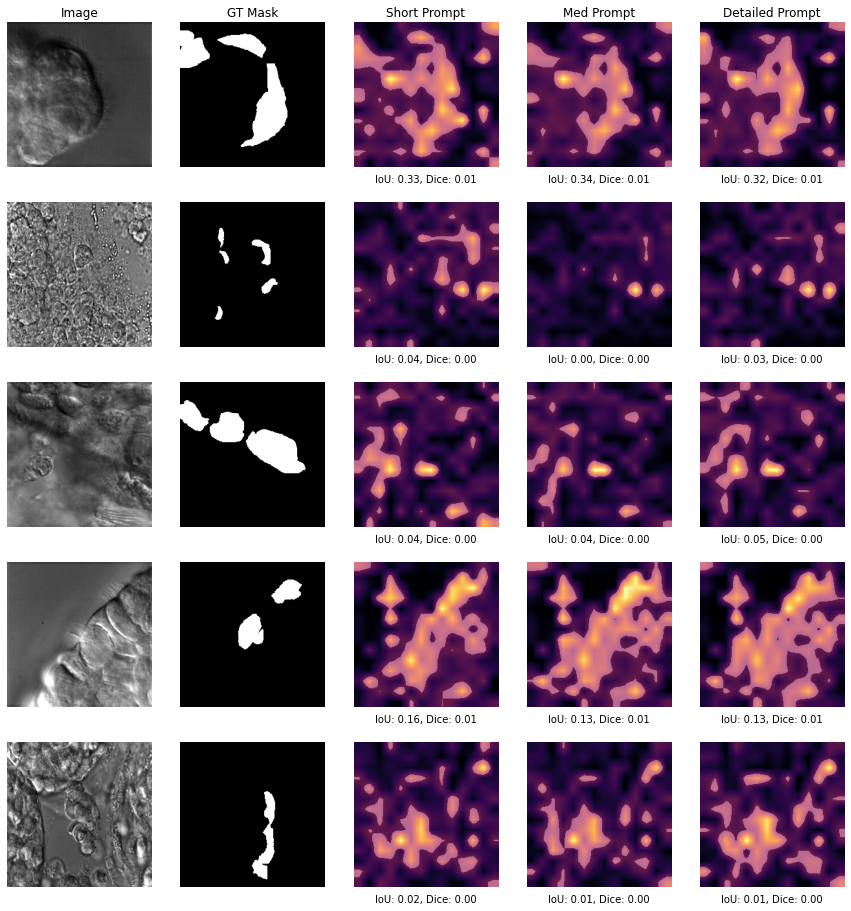
\includegraphics[width=\textwidth]{figures/sam/fine-tuned masks long captions small train 01 09 095 005.png} % Caption below suggests beta=0.65, 0.65 but filename suggests 0.95, 0.05. Assuming caption reflects the specific experiment shown.
    \caption{Impact of adjusted hardness parameters (\(\beta_1=0.65\), \(\beta_2=0.65\)) during fine-tuning, showing improved localization diversity but potentially higher false-positive rates compared to baseline fine-tuning.}
    \label{fig:fine_tuned_masks_small_train_01_09_095_005} % Label might need alignment with caption/experiment if filename is misleading.
\end{figure}

\begin{table}[ht]
    \centering
    \caption{Average IoU and Dice scores of BiomedCLIP models under different training configurations}
    \label{tab:biomedclip_performance}
    \renewcommand{\arraystretch}{1.2}
    \begin{tabular}{|l|c|c|}
        \hline
        \textbf{Model Variant}                                          & \textbf{Average IoU} & \textbf{Average Dice} \\ \hline
        Un-tuned BiomedCLIP (zero-shot)                                 & 0.092                & 0.0033                \\ \hline
        Fine-tuned for 32 epochs on full images (overfit)               & 0.000                & 0.0000                \\ \hline
        Fine-tuned \(\tau=0.1, \alpha=0.9, \beta_1=0.95, \beta_2=0.05\) & 0.106                & 0.0040                \\ \hline
    \end{tabular}
    % \par\medskip
    % \footnotesize *Configuration uses masked images, 5 epochs, trained on long captions.
\end{table}

\subsection{Impact of Fine-tuning BiomedCLIP}

Our fine-tuning experiments revealed that performance improvements are highly dependent on the specific training conditions. Fine-tuning BiomedCLIP using full-sized, raw images proved detrimental, severely impairing the model's localization capabilities regardless of the number of training epochs, likely due to the model failing to focus on relevant features amidst complex backgrounds. Conversely, fine-tuning using masked images, which isolate the cell bodies and ciliary structures, consistently improved localization accuracy by focusing the model's learning process. However, training beyond an optimal number of epochs (empirically found to be around 5 epochs for configurations using masked images) did not enhance performance further. Instead, extended training introduced overfitting and degraded generalizability, as indicated by the increasingly sparse and overly specialized activation maps shown for a 32-epoch run in Figure \ref{fig:fine_tuned_no_mask_ep32}.

A quantitative assessment using per-pixel confusion matrix metrics (Table \ref{tab:confusion_matrix_avg}) further elucidates the impact of fine-tuning. Compared to the untuned model, the fine-tuned version (using the configuration specified in Table \ref{tab:biomedclip_performance}) demonstrated improved sensitivity, achieving higher average True Positive (TP) counts and lower average False Negative (FN) counts across Short, Medium, and Detailed prompts. This confirms the fine-tuned model's enhanced ability to correctly identify actual positive pixels (cilia). However, this gain in sensitivity was accompanied by a significant reduction in specificity, evidenced by the substantial increase in average False Positive (FP) counts and the corresponding decrease in average True Negative (TN) counts. This indicates the fine-tuned model became more liberal in its classifications, incorrectly labeling a larger number of background pixels as positive. Notably, the performance variation across different prompt types appeared less pronounced in the fine-tuned model compared to the untuned one based on these metrics.

\begin{table}[htbp]
    \centering
    \caption{Average Per-Pixel Confusion Matrix Metrics (15 Test Samples)}
    \label{tab:confusion_matrix_avg}
    \begin{tabular}{llcccc} % Removed unnecessary vertical lines for booktabs style
        \hline
        Model Type & Prompt Type & Avg. TP & Avg. TN  & Avg. FP & Avg. FN \\
        \hline
        Untuned    & Short       & 1370.60 & 43288.20 & 2802.40 & 2714.80 \\
                   & Medium      & 1203.40 & 43001.00 & 3089.60 & 2882.00 \\
                   & Detailed    & 1642.80 & 42078.60 & 4012.00 & 2442.60 \\
        \hline
        Fine-tuned & Short       & 1839.80 & 37405.00 & 8685.60 & 2245.60 \\
                   & Medium      & 1669.80 & 37407.60 & 8683.00 & 2415.60 \\
                   & Detailed    & 1713.20 & 37208.80 & 8881.80 & 2372.20 \\
        \hline
    \end{tabular}
    \par\medskip
    \footnotesize
    Note: TP = True Positives, TN = True Negatives, FP = False Positives, FN = False Negatives. Values represent average per-pixel counts over 15 test samples. Fine-tuned model corresponds to the configuration: \( \tau = 0.1 \), \( \alpha = 0.9 \), \( \beta_1 = 0.95 \), \( \beta_2 = 0.05 \), masked images, 5 epochs, trained on long captions.
\end{table}

\subsection{Effects of Textual Prompts}

\begin{table}[htbp]
    \centering
    \caption{Caption Generation Logic Based on Image Content for Fine-Tuning.}
    \label{tab:caption_generation_logic}
    \small
    \begin{tabular}{p{3cm}p{5cm}p{7cm}} % Removed vertical lines
        \toprule % Use booktabs style
        \textbf{Image Content}      & \textbf{Short Caption}                                                                                                                                                                                   & \textbf{Long Caption}                                                                                                                                                                                                                                                                                                                                                                                                                                                                \\
        \midrule
        Masked Cell Body (No Cilia) & \textbf{Fixed text:} \texttt{nasal epithelial cell}                                                                                                                                                      & \textbf{Fixed text:} \texttt{a microscopy image of nasal epithelial biopsy containing epithelial cell}                                                                                                                                                                                                                                                                                                                                                                               \\
        \addlinespace % Requires booktabs
        Masked Ciliary Region       & \textbf{Generated based on the source video's label (motile, immotile, or indeterminate):} Resulting text is like \texttt{"normal cilia"}, \texttt{"abnormal cilia"}, or \texttt{"indeterminate cilia"}. & \textbf{Generated based on source video label and mask analysis:} Starts with \texttt{"nasal epithelial biopsy of [\textit{state}] cilia..."} (where \textit{state} reflects motile/immotile/indeterminate). Continues by describing visibility based on mask characteristics, using phrases like \texttt{"...exposed and clearly visible protruding out..."} for easily detected cilia, or \texttt{"...overlaying the body of the cell and are hard to detect"} for obscured cilia. \\
        \bottomrule % Use booktabs style
    \end{tabular}
    \par\medskip
    \footnotesize
    Note: If both clearly visible and hard-to-detect cilia are present according to the mask analysis, the long caption explicitly mentions this mixed visibility (e.g., "...some cilia protrude... clearly visible, while some other cilia are overlaying... hard to detect."). Additionally, to enhance diversity, the exact phrasing and use of synonyms within the descriptive parts of the long captions were randomized during generation.
\end{table}

The nature of textual prompts used during fine-tuning and inference also significantly impacted model performance (details of caption generation logic are in Table \ref{tab:caption_generation_logic}). Our experiments showed that employing short, concise textual prompts generally led to more consistent localization with fewer false-positive results, particularly when the model was also trained using corresponding short captions. Conversely, utilizing longer, more detailed prompts and captions (as seen in Figure \ref{fig:train_long_captions}) could introduce ambiguity, sometimes increasing the incidence of both false positives and false negatives. A crucial observation was the importance of consistency between training captions and inference prompts: models trained with brief captions performed best with brief prompts, whereas models trained on detailed captions benefited from detailed prompts during inference.

\subsection{Hyperparameter Optimization and Stability}

Exploration of the DHN-NCE loss hyperparameters revealed nuances in their influence on stability and accuracy. Within a moderate range, variations in the hardness weighting parameters \( \beta_1 \) and \( \beta_2 \) showed minimal impact. However, employing more extreme, asymmetric values (such as \( \beta_1 = 0.95, \beta_2 = 0.05 \), used in the primary fine-tuned configuration reported in Tables \ref{tab:biomedclip_performance} and \ref{tab:confusion_matrix_avg}) significantly heightened the model's sensitivity to differences in textual prompts, potentially leading to instability. Separate experiments indicated that a balanced beta configuration (e.g., \( \beta_1 = 0.65, \beta_2 = 0.65 \)), particularly when combined with long captions during training (as illustrated in Figure \ref{fig:fine_tuned_masks_small_train_01_09_095_005}), could offer a good trade-off by maximizing detection accuracy while potentially mitigating some false positives compared to the more sensitive configuration. Adjusting the temperature parameter \( \tau \) also had effects; higher temperatures led to smoother, more blurred similarity distributions, which could compromise localization precision.
% (Figure \ref{fig:fine_tuned_with_mask_th_0_4}).

\subsection{Prompt Selection Strategies for SAM}

Finally, our analysis underscored the critical importance of how BiomedCLIP-generated saliency maps are translated into spatial prompts for the downstream SAM model. We found that common strategies, such as randomly selecting points solely from the largest detected contour in the thresholded map, were often inadequate, especially for ROIs like cilia that can be sparse and distributed across multiple small regions. Our findings emphasize that more nuanced approaches, which consider multiple salient contours or employ different heuristics based on the map's characteristics, can significantly enhance segmentation accuracy, particularly for complex images with overlapping or indistinct ROIs.

\section{Conclusion and Final Remarks}

This chapter investigated the application of foundation models for biomedical image segmentation, focusing specifically on optimizing the BiomedCLIP vision-language model to generate high-quality saliency maps intended as input for a downstream Segment Anything Model (SAM). Our work, centered on the challenging task of ciliary region identification, highlighted the limitations of traditional methods and explored how fine-tuning a vision-language model can enhance the initial, prompt-generation stage of a SAM-based segmentation pipeline.

A key finding is the observed performance difference in BiomedCLIP before and after fine-tuning for this specialized task. Our baseline evaluation showed that the off-the-shelf BiomedCLIP model demonstrated limitations in localization accuracy (e.g., low average IoU scores, high false negatives) and produced inconsistent saliency maps across different prompt types (Table \ref{tab:biomedclip_performance}, Table \ref{tab:confusion_matrix_avg}). In contrast, strategic fine-tuning resulted in an improvement in BiomedCLIP's ability to generate stable and accurate saliency maps relevant to the target structures. Although this fine-tuning increased sensitivity (higher True Positives, lower False Negatives), it also reduced specificity, evidenced by the increase in average False Positive counts (Table \ref{tab:confusion_matrix_avg}). This observed contrast underscores the necessity of domain-specific adaptation for vision-language models when preparing inputs for subsequent segmentation tasks in specialized biomedical contexts.

Our investigations demonstrated that the effectiveness of BiomedCLIP fine-tuning is highly sensitive to the chosen methodology. We found that minimal fine-tuning (e.g., around 5 epochs) using masked images and concise textual prompts often yielded robust saliency maps. This effectiveness likely stems from several factors: using masked images focuses the model on relevant features; shorter training durations prevent overfitting, promoting generalization; and concise prompts provide a clearer, less ambiguous signal to the model.

The refined saliency maps generated by the optimally tuned BiomedCLIP serve as a more effective foundation for deriving precise spatial prompts (points or bounding boxes) intended for use with SAM. The experiments underscored the importance of the prompt selection method, showing that simplistic strategies (like selecting random points from only the largest contour) are not universally optimal, especially for sparse or distributed ROIs where multi-contour strategies are preferable. The effectiveness of any prompt selection strategy is intrinsically linked to the quality and characteristics of the saliency map produced by the fine-tuned vision-language model.

Furthermore, while this work focused primarily on optimizing and understanding the reproducibility of the prompt generation stage via BiomedCLIP, achieving reliable end-to-end segmentation necessitates acknowledging factors beyond this scope. Potential stochasticity within SAM's internal mask decoding process or implementation variations could still affect final segmentation reproducibility even with identical input prompts, representing an area for future investigation relevant to the broader goal of creating robust biomedical tools. Our results, focused on improving the input to SAM, indirectly support the notion that an off-the-shelf SAM could be utilized more effectively when provided with high-quality, targeted prompts derived from a well-tuned upstream model, particularly for tasks where ROIs are clearly indicated by the prompts. However, the question of whether SAM itself requires fine-tuning for optimal performance across diverse biomedical conditions remains an open area addressed by other studies in the field.

In conclusion, a carefully fine-tuned vision-language model, configured with optimized parameters and training strategies, coupled with intelligent, context-aware selection of spatial prompts derived from its output, enhances the potential for effective segmentation using an off-the-shelf SAM by providing it with improved guidance. Future work stemming from this investigation should focus on the prompt generation and selection process:
\begin{itemize}
    \item Developing more sophisticated, adaptive, and potentially automated spatial prompt selection algorithms that optimally leverage the information in the refined saliency maps, tailored to specific biomedical imaging characteristics and ROI distributions.
    \item Exploring advanced fine-tuning techniques (e.g., parameter-efficient methods) specifically for the vision-language model (BiomedCLIP) to further optimize saliency map quality and stability.
    \item Investigating how variations in the quality and type of prompts generated by different BiomedCLIP configurations influence the downstream performance and behavior of a fixed SAM model.

\end{itemize}
By improving the crucial link between textual/visual understanding (BiomedCLIP) and spatial segmentation (SAM), such advancements will contribute to realizing more robust, reliable, and clinically valuable biomedical image segmentation frameworks that leverage the power of foundation models.

% \section{Conclusion and Final Remarks}

% This chapter investigated the application of foundation models, specifically the combination of BiomedCLIP and SAM, to the challenging task of biomedical image segmentation, using ciliary region identification as a case study. We highlighted the limitations of traditional supervised and unsupervised methods and positioned foundation models as a promising alternative due to their zero-shot or few-shot capabilities facilitated by user prompts.

% Our investigations demonstrated that while off-the-shelf vision-language models like BiomedCLIP may struggle with specialized biomedical targets, strategic, minimal fine-tuning significantly improves the stability and accuracy of the generated saliency maps. These refined maps provide a more reliable foundation for generating precise spatial prompts (points or bounding boxes) required by SAM. The experiments clearly underscored the criticality of the prompt generation method itself, revealing that simplistic approaches (like using only the largest contour) are not universally optimal, especially for sparse or distributed ROIs where multi-contour strategies yield better results. The effectiveness of any prompt selection strategy is intrinsically linked to the quality and characteristics of the saliency map produced by the (fine-tuned) vision-language model.

% Furthermore, our findings suggest that SAM itself can be effective off-the-shelf for certain biomedical tasks, provided the ROIs are well-defined, enclosed, and relatively free of artifacts. However, achieving consistent reliability across the diverse and complex range of biomedical imaging modalities and conditions often necessitates fine-tuning of the segmentation model (SAM) in addition to optimizing the prompt generation stage.

% In conclusion, a carefully fine-tuned vision-language model coupled with intelligent, context-aware selection of spatial prompts considerably enhances the segmentation capabilities of models like SAM in the biomedical domain. Future work should focus on developing more sophisticated and adaptive prompt selection strategies tailored to specific biomedical imaging characteristics and target structures. Such advancements, potentially combined with efficient fine-tuning techniques for SAM itself, will be crucial in realizing the full potential of foundation models for robust, reliable, and generalizable biomedical image segmentation.


\end{document}